\title{Dot Products and Length}
\subtitle{\SubTitleName}
\institute[]{\Course}
\author{\Instructor}
\maketitle   
  


\tikzstyle{row} =[rectangle, minimum width=2cm, minimum height=2cm, text centered, fill=red!30,draw=green, rotate=45]

\tikzstyle{col} = [rectangle, minimum width=2cm, minimum height=2cm, text centered, fill=red!30,draw=green, rotate=135]

\tikzstyle{nul} = [trapezium, trapezium left angle=90, trapezium right angle=90, minimum width=1cm, minimum height=1cm, text centered, rotate=140]

\tikzstyle{left} = [trapezium, trapezium left angle=90, trapezium right angle=90, minimum width=1cm, minimum height=1cm, text centered, rotate=30]

\tikzstyle{arrow} = [thick,->,>=stealth]




\frame{\frametitle{Topics and Objectives}
\Emph{Topics} \\
%\TopicStatement
\begin{itemize}

    \item dot products

    \item magnitude of vectors
    
    \item distances in $\mathbb R^n$ 
    
    \item angles between vectors

    % \item Orthogonal vectors and complements
    

\end{itemize}

\vspace{0.5cm}

\Emph{Learning Objectives}\\

\LearningObjectiveStatement

\begin{itemize}

    \item characterize relationships between vectors using the (a) dot product of two vectors, (b) length (or magnitude) of a vector, (c) distance between points in $ \mathbb R^n$, and (d) angles between vectors
    
    % \item Apply theorems related to orthogonal complements, and their relationships to Row and Null space, to characterize vectors and linear systems.
\end{itemize}

} 




\begin{frame}\frametitle{The Dot Product} 

    The dot product between two vectors, $\vec u$ and $\vec v$ in $\mathbb R^n$, is defined as
    \pause 
    \vspace{-4pt}
    \begin{equation*}
    \vec u \cdot \vec v = \vec u \, ^T \vec v = 
    \begin{pmatrix*}[r]
    u_1 & u_2 & \cdots & u_n 
    \end{pmatrix*} 
    \begin{pmatrix*}[r]
    v_1 \\ v_2 \\ \vdots \\ v_n
    \end{pmatrix*} = u_1 v_1 + u_2 v_2 + \cdots + u_n v_n . 
    \end{equation*}
    
    \pause 
    
    \Emph{Example:} For what values of $k$ is $ \vec u \cdot \vec v=0$?
    
    $$\vec u = \spalignmat{ -1 ;  k; 2}, \qquad \vec v = \spalignmat{4 ;1; 3}$$

\end{frame}




\begin{frame} \frametitle{Theorem: Dot Product Identities}

    % The dot product is a special form of matrix multiplication, so it inherits its properties.  

    % \begin{center}\begin{tikzpicture} \node [mybox](box){\begin{minipage}{0.95\textwidth}
    % \vspace{4pt}
        Let $ \vec u, \vec v, \vec w$ be three vectors in $ \mathbb R ^{n}$, and $c \in \mathbb R$. 
        \begin{align*}
            \onslide<2->{(\vec v + \vec w) \cdot \vec u & = \vec v \cdot \vec u + \vec w \cdot \vec u && linearity } \\ 
            \onslide<3->{(c \vec u) \cdot \vec w &= c (\vec u \cdot \vec w) && scalars } \\ 
            \onslide<4->{\vec u \cdot \vec w &= \vec w \cdot \vec u  &&  symmetry } \\
            \onslide<5->{\vec u \cdot \vec u & \geq  \, 0 && positivity  } \\
            \onslide<6->{\vec u \cdot \vec u &= 0 \Leftrightarrow \vec u = \vec 0}
        \end{align*}

    % \end{minipage}};
    % \node[fancytitle, right=10pt] at (box.north west) {};
    % \end{tikzpicture}\end{center}



\end{frame}



\begin{frame}\frametitle{The Length of a Vector}

    % ~~ ~~ Highlight Box ~~ ~~
    \begin{center}\begin{tikzpicture} \node [mybox](box){\begin{minipage}{0.85\textwidth}\vspace{4pt}

        The \Emph{length} of a vector $\vec u \in \mathbb R^n$ is  \begin{equation*}
            \lVert \vec u\rVert = \sqrt { \vec u \cdot \vec u} = 
            \sqrt {  u_1 ^2 + u_2 ^2 + \cdots + u_n ^2 }
        \end{equation*}

    \end{minipage}};
    \node[fancytitle, right=10pt] at (box.north west) {Definition};
    \end{tikzpicture}\end{center}
    % ~~ ~~ Highlight Box ~~ ~~
    \vspace{-12pt}
    \begin{columns}
    \begin{column}{.55\textwidth}
    
    \pause 
    
    \Emph{Example} \\ If $P$ is the point $(1,3,2)$, the length of vector $\overrightarrow{OP}$ is $$\sqrt{1^2 + 3^2 + 2^2} = \sqrt{14}$$
    
    \end{column}\begin{column}{.4\textwidth}
    
        \begin{center}
        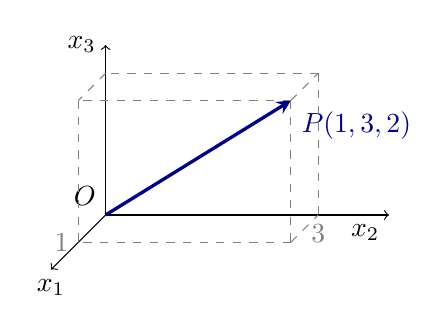
\begin{tikzpicture}[scale=0.9, axis/.style={->,black}, 
            vector/.style={-stealth,DarkBlue,very thick}, 
            vector guide/.style={dashed,gray}]
    
            \coordinate (P) at (3,2,1);
            \coordinate (O) at (0,0,0);
    
            %draw axes
            \draw[axis] (0,0,0) node[anchor=south east]{$O$} -- (4,0,0) node[anchor=north east]{$x_2$};
            \draw[axis] (0,0,0) -- (0,2.4,0) node[anchor=east]{$x_3$};
            \draw[axis] (0,0,0) -- (0,0,2) node[anchor=north]{$x_1$};
            \draw[vector] (O) -- (P) node[anchor=north west]{$P(1,3,2)$};
    
            \draw[vector guide] (3,0,1) -- (3,0,0) node[anchor=north]{$3$};
            \draw[vector guide] (3,0,1) -- (0,0,1) node[anchor=east]{$1$};
            \draw[vector guide] (3,2,1) -- (3,0,1);
            \draw[vector guide] (3,2,1) -- (0,2,1);
            \draw[vector guide] (3,2,1) -- (3,2,0);
            \draw[vector guide] (3,2,0) -- (0,2,0);
            \draw[vector guide] (0,2,0) -- (0,2,1);
            \draw[vector guide] (0,2,1) -- (0,0,1);
            \draw[vector guide] (3,2,0) -- (3,0,0);
        \end{tikzpicture}        
        \end{center}
    
    
    \end{column}
    \end{columns}

    



    




\end{frame}
 


\begin{frame} \frametitle{Example}

    Let $ \vec u, \vec v$ be two vectors in $ \mathbb R ^{n}$ with $ \lVert \vec u\rVert=5 $, $ \lVert \vec v\rVert=\sqrt 3$, and $ \vec u \cdot \vec v = - 1$. Compute the value of $ \lVert \vec u + \vec v\rVert$.  

\end{frame}





\begin{frame}\frametitle{Length of Vectors and Unit Vectors}

    \Emph{Note}: for any vector $ \vec v$ and scalar $c$, the length of $ c \vec v$ is %$ \lVert c\vec v\rVert= \lvert  c\rvert \cdot \lVert \vec v\rVert $.  
    \begin{equation*}
        \lVert c\vec v\rVert = |c| \, ||\vec v||
    \end{equation*}
    
    % ~~ ~~ Highlight Box ~~ ~~
    \begin{center}\begin{tikzpicture} \node [mybox](box){\begin{minipage}{0.85\textwidth}\vspace{2pt}

        If $ \vec v \in \mathbb R^n$ has length one, we say that it is a \Emph{unit vector.} 

    \end{minipage}};
    \node[fancytitle, right=10pt] at (box.north west) {Definition};
    \end{tikzpicture}\end{center}
    % ~~ ~~ Highlight Box ~~ ~~
    

    \vspace{6pt}
    
    \pause

    For example, each of the following vectors are unit vectors.  
    \begin{align*}
        \vec e_1 = \spalignmat{1;0} , \quad
        \vec y = \frac{1}{\sqrt 5}\spalignmat{1;2} , \quad 
        \vec v = \frac{1}{\sqrt 3}\spalignmat{1;0;1;1}
    \end{align*}

\end{frame}
 
 
 
 
 
 
 
\begin{frame}\frametitle{Distance in $ \mathbb R ^{n}$} 

    % ~~ ~~ Highlight Box ~~ ~~
    \begin{center}\begin{tikzpicture} \node [mybox](box){\begin{minipage}{0.8\textwidth}\vspace{2pt}

        For $ \vec u, \vec v \in \mathbb R ^{n}$, the \Emph{distance} between $ \vec u$ and $ \vec v$ is given by the formula $||\vec u - \vec v ||$. 

    \end{minipage}};
    \node[fancytitle, right=10pt] at (box.north west) {Definition};
    \end{tikzpicture}\end{center}
    % ~~ ~~ Highlight Box ~~ ~~
    
    \pause
    
    \Emph{Example:}
    Compute the distance from $ \vec u = \spalignmat{7;1}$ and $ \vec v = \spalignmat{3;2}$. 
    \begin{center}
        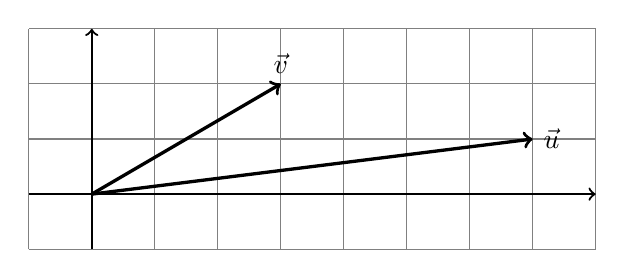
\begin{tikzpicture}[yscale=.7,xscale=.8] 
            \draw[gray](-1,-1) grid (8,3);  
            \draw[->,thick]  (-1,0) -- (8,0); 
            \draw[->,thick]  (0,-1) -- (0,3); 
            \draw[->,black,very thick] (0,0) -- (7,1) node[right] {$ \vec u$}; 
            \draw[->,black,very thick] (0,0) -- (3,2) node[above] {$ \vec v$}; 
        \end{tikzpicture}
    \end{center} 


\end{frame}


\begin{frame}\frametitle{Angles}
    
    \begin{center}
    \begin{tikzpicture} \node [mybox](box){\begin{minipage}{0.65\textwidth}
        \vspace{2pt}
        
        $ \vec a \cdot \vec b= ||\vec a|| \, ||\vec b|| \,  \cos\theta$. Thus, if $\vec a \cdot \vec b = 0$, then: 
        \begin{itemize} \setlength\itemsep{0.25em}
            \item<2-> $ \vec a$ and/or $ \vec b$ are zero vectors, or 
            \item<3-> $ \vec a$ are $ \vec b$ are perpendicular to each other. % orthogonal 
        \end{itemize}

        \end{minipage}};\node[fancytitle, right=10pt] at (box.north west) {Theorem};
    \end{tikzpicture}
    \end{center}

    \onslide<4->{
    For example, consider the vectors below.
    
     \begin{center}
        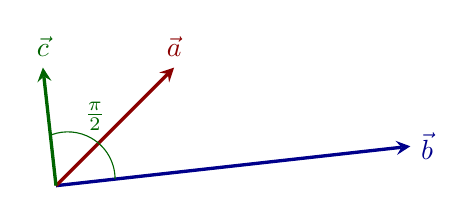
\begin{tikzpicture}[scale=0.5] 
            \draw[->,DarkBlue,very thick,-stealth] (0,0) -- (9,1) node[right] {$ \vec b$}; 
            \draw[->,DarkRed,very thick,-stealth] (0,0) -- (3,3) node[above] {$ \vec a$}; 
            \draw[->,DarkGreen,very thick,-stealth] (0,0) -- (-3/9,3) node[above] {$ \vec c$}; 
            % \draw[DarkRed] (2,2/9) arc (0:58:1.3) node[midway, right] {$\theta$};            
            \draw[DarkGreen] (1.5,0.1666) arc (0:110:1.2) node[midway, above] {$\frac{\pi}{2}$};            
        \end{tikzpicture}
    \end{center} 
    }
    
\end{frame}



\frame{\frametitle{Summary}

    \SummaryLine \vspace{4pt}
    \begin{itemize}\setlength{\itemsep}{8pt}

    \item dot products

    \item magnitude of vectors
    
    \item distances in $\mathbb R^n$ 
    
    \item angles between vectors
    
    \end{itemize}
    
    \vspace{8pt}
    
}


